\documentclass{template/abschlussarbeit}

%%%%%%%%%%%%%%%%%%%%%%%%%%%%%%%%%%%%%%%%%%%%%%%%%%%%%%%%%%%%
% Allgemeine Variablen fuer die Abschlussarbeit (mit eigenen
% Angaben ausfuellen!)
%%%%%%%%%%%%%%%%%%%%%%%%%%%%%%%%%%%%%%%%%%%%%%%%%%%%%%%%%%%%

\AutorVorname{Sven}
\AutorNachname{Gasterstädt}
\AutorGeburtsort{Wuppertal}
\AbschlussarbeitTitel{Efficient Importing and Loading of Various Graph File Formats into a Distributed In-Memory System}
% Bachelorarbeit, Projektarbeit, Masterarbeit
\AbschlussarbeitTyp{Bachelorarbeit}
% keywords durch , getrennt
\AbschlussarbeitKeywords{Distributed Systems, Big Data, Graph File Formats, Loading, Parsing}
\Ort{Düsseldorf}
\Datum{15.03.2019}
\Erstgutachter{Prof. Dr. Michael Schöttner}
\Zweitgutachter{Prof. Dr. Stefan Conrad}
\Betreuer{Prof. Dr. Michael Schöttner}

% Hier den vollstaendigen Dateinamen der bibtex Datei angeben
% Falls diese in einem Unterordner liegt, so ist dieser relativ
% zu dieser Datei (document.tex) anzugeben.
\LiteraturBibtexDatei{library}

% Der Anhang (falls vorhanden) wird hier genauso wie diese
% Bibtex-Datei angegeben (jedoch ohne .tex-Endung!)
\AnhangDatei{chap/anhang}

%%%%%%%%%%%%%%%%%%%%%%%%%%%%%%%%%%%%%%%%%%%%%%%%%%%%%%%%%%%%
% Optionen/Schalter um bestimmte Abschnitte an-/auszuschalten
% WICHTIG: Nicht genutzte/leere Abschnitte vor der Abgabe/
% dem finalen Druck abschalten durch auskommentieren.
% Gleiches gilt fuer die Todo Liste, welche nicht in die 
% finale Version gehoert.
%%%%%%%%%%%%%%%%%%%%%%%%%%%%%%%%%%%%%%%%%%%%%%%%%%%%%%%%%%%%

\Titelblatt
\Inhaltsverzeichnis
\Abbildungsverzeichnis
\Tabellenverzeichnis
\Algorithmenverzeichnis
\Anhang
\Erklaerung

%%%%%%%%%%%%%%%%%%%%%%%%%%%%%%%%%%%%%%%%%%%%%%%%%%%%%%%%%%%%h
\begin{document}
\begin{abschlussarbeit}

%%%%%%%%%%%%%%%%%%%%%%%%%%%%%%%%%%%%

% Hier werden die einzelnen Kapitel aufgelistet (Reihenfolge!)
% Die vorgegebenen Kapitel dienen als Hilfestellung waehrend der Arbeit
% und sind mit der Fertigstellung des finalen Dokuments zu entfernen!

\chapter{Introduction}
\label{Introduction}

With the growing amount of generated data, the size of files is increasing as well. It is an important topic to deal with the problem of efficient loading and importing, especially in times of big data where file sizes of several gigabytes are common. Also each second of high-performance computing is very valuable and in many cases algorithms can not proceed with an incomplete dataset. This results in long waiting times, while the loading task is running.\\
The data is often stored in graph like networks, where data is represented by vertices and edges. These graphs can consist of billions of small objects, in which case the meta data overhead must be very small to work efficiently. There are many kinds of various graph file formats but this thesis will only focus on the most common and relevant ones, which serve the purpose of exchange the information between two systems.\\\\
This works tries to resolve the problems, which comes with trying to use the resources of a distributed system to accelerate the loading of graphs into memory and manage the chunk distribution in the network. To accomplish this the file format must be parallelizable. This needs to be determined first. The graph files formats, this work deals with, will be evaluated to their parallelizability, their relevance and current state of use. Over the course of time various graph file formats got introduced with many different properties and purposes. They vary from simple edge lists to complex formats in binary or xml format.\\\\
The current state-of-the-art standard is that a parallelizable file format gets used and mapped on a map-reduce framework. Therefor often simple formats are used, like neighbor lists, where the overhead to deal with is very small and one line describes exactly one node and its edges. It's common practice that complex formats get parsed into simpler ones and then read in. This work will try to accomplish a map-reduce-like approach with many more formats, while trying to preserve the performance gained by the resources of a distributed system.

\chapter{Preliminaries}
\label{Preliminaries}
\section{Graph File Formats}
A graph file format is a specification for describing a graph in a predefined syntax, which then can be read in by an application to access the data. Over the course of time many graph file formats have been established. Most of these formats were developed, with special use cases in mind. For example GraphML was designed to support as many features as possible for graph drawing\cite{Roughan.10.03.2015}.
In the recent time the trend to invent new graph formats is decreasing. It can be seen  that most of the formats are not developed any further, also there is an significant reduction of XML type formats in the last couple of years and the number of JSON graph file formats is rising\cite{Roughan.10.03.2015}.
Based on the collection provided in \cite{Roughan.10.03.2015}, a table with formats was created to identify their up-to-dateness.

\begin{table}[H]
\begin{center}
		\caption{Selection of up-to-date Graph File Formats based on \cite{Roughan.10.03.2015}}
    \begin{tabular}{| l | l | l | l |}
    \hline
	\bfseries Id & \bfseries Graph file format & \bfseries Reference time frame & \bfseries Structure\\ \hline
	1 & GraphML & 2000 - present & XML\\ \hline
	2 & JSON Graph & 2014 - present & JSON\\ \hline
	3 & KrackPlot & 1993 - present & simple\\ \hline
	5 & Ordered Graph Data Language & 2002 - present & BNF\\ \hline
	6 & Open Graph Markup Language & 2012 - present & XML\\ \hline
	7 & Simple Interaction Format & 2003 - present & simple\\ \hline
	8 & Stanford Network Analysis Platform & 2005 - present & simple\\ \hline
	9 & Text Encoding Initiative Graph Forma & 2001 - present & XML\\ \hline 
	10 & Trival Graph Format & unknow - present & simple\\ \hline

    \end{tabular}
\end{center}
\label{tabelle_avarage_time.10}
\end{table}
 There are several properties, which a graph file format has to fulfill. For example, not all formats are a good option for big data sets. XML and even JSON formats have an bigger overhead then just a simple edge list \cite{JSONvsXML.10}. This overhead scales with the size of the data and can have an impact on the performance of the loading. Our file formats have to be scalable, otherwise just small datasets can be supported and this results in probably faster loading times on a single peer. Most big data sets are provided in simple formats and resolve around keeping the overhead small. But at the same time these formats try to be as simple as possible.
 Also there file formats that do not provide any clear specifications or the development has been stopped. This is a problem with more complex formats, because this problem could lead to inconsistencies while loading or reading these format files. 
 For more simple formats are often no specifications needed, because they follow a trivial approach. This simplicity makes them self-explanatory.

\subsection{Division of Formats}
To enable distributed loading, the graph file format needs to be split into multiple chunks \cite{parallelGraphLoading.10}, which then can be distributed inside the distributed system. The goal is to gain performance, while processing the data parallel on multiple nodes. To be able to split the file, an section must be identified, so that the information inside these chunks does not lose it current context. A chunk without its context, can not be interpreted correctly and will unavoidable lead to an wrong graph. If the context is not keep-able, than loading the format on a single node is probably the best workaround.\\
It is not surprising that most formats are divisible in some way, but the main factor to consider at this point, is performance. All peers must wait for the chunks to be created, that is why in this step no interpretation of the file should be done. This is not avoidable for all formats, but for the most simple formats there is a way split files without or minimal reading of the file itself.\\
To determine if a format is divisibility, the structure of the file needs to be specified and analyzed. Most important data inside the file should not be dependent on other sections of the same file. In other words the chunks should contain all needed data for reading. 
There will be formats that specify information about vertices in multiple sections of the file, but this information needs to be independent. If the following data can only be processed after processing all lines before, then this section can not be split. Sections that can not be split for example are edge-tuples. This sections will be referred as indivisible sections.\\
These indivisible sections are often surrounded or closed by separators. A separator could be anything. For example newline characters, tabulations and  semicolons are often used, but also tags (XML), brackets (JSON) or even the position itself in binary sequences can be used to divide these sections. Some formats provide meta data, that will help split up files by defining the position of the information and their format.\\
A format is fully divisible if it could be split at any separator. This will mostly be true for simple formats.

\newpage
\subsection{Simple Formats}
Simple formats are often a trivial approach of creating a low level but highly functional graph file format. These formats are often self-explanatory, but have no official specification. This leads to various problems, because it is not clear where the boundaries of this formats are. For example the information of the used character set or separators is missing. Also it is not always stated if the format contains meta data or comments\cite{Roughan.10.03.2015}.\\
Many of these formats are fully divisible, due to the fact that they often only contain small indivisible sections. These sections can be grouped and stored in chunks. Also leads their simple structure to a plain hierarchy inside the file.

\subsubsection{Trivial Graph Formats}
As trivial graph file formats (TGF) are referred to a list of formats, that follows a simple implementation but have no specification. The most common formats are standard approaches like edge lists, adjacency matrices, neighbor lists and path list.\\

\noindent{\textit{Edge List}}\\
The Edge list is the most common and trivial approach of storing a graph.
This format is just a list of all edges of the graph.
One line represents one edge and is represented by two vertices. Each line forms an indivisible section, after which the file could be split. The vertices of an edge are split by a separator. Often tabulations are used here, but also spaces and other characters can be used (e.g ~\ref{edgeEx}). This format has a relatively low overhead and scales well.
\vspace{-7mm}
\begin{center}
	\begin{minipage}{.6\textwidth}
\begin{lstlisting}[numbers=left,firstnumber=1,caption={Edge List},captionpos=b,linewidth={\textwidth}, escapeinside=||,label={edgeEx}]
|$v_1$| |$v_2$|
|$v_1$| |$v_3$|
|$v_2$| |$v_3$|
\end{lstlisting}
\end{minipage}
\end{center}


\noindent{\textit{Binary Edge List}}\\
The Binary Edge List is a compressed version of the Edge List, where no lines are used, instead all edges have a fixed size. For example an edge is represented by a start vertex and a target vertex. Vertices are written in this case as eight bytes each, so the first eight bytes indicate the start vertex and the following eight bytes the target vertex (e.g ~\ref{BedgeEx}). This compression leads to the advantage that no separator is used. The Binary Edge List has no overhead, but the human readability is lost. This format scales especially well for big graphs and is simple to read in.
\vspace{-7mm}
\begin{center}
	\begin{minipage}{.6\textwidth}
\begin{lstlisting}[numbers=left,firstnumber=1,caption={Binary Edge List in Hex View},captionpos=b, linewidth={\textwidth}, escapeinside=||, breakindent=0pt,	
breaklines=true,label={BedgeEx}]
|$0000000000000001_{16}$||$0000000000000002_{16}$||$0000000000000001_{16}$| |$0000000000000003_{16}$||$0000000000000002_{16}$||$0000000000000003_{16}$| ...|$v_{1}v_{2}v_{1}v_{3}v_{2}v_{3}$|
\end{lstlisting}
\end{minipage}
\end{center}
\newpage
\noindent{\textit{Adjacency Matrix}}\\
The Adjacency Matrix is a format, which is based on a adjacency matrix. Each entry in this matrix represents an edge connection between the vertex, which are identified through the row and column number. Often the row and column numbers are not written in the file and the parser has to keep track of them (e.g ~\ref{AdjMat}). The biggest flaw of this format is that it does not scale well for big data sets, due to the fact that every vertex got an entry for all other vertices. So its size increases squarely to the amount of vertices of the graph.
\vspace{-7mm}
\begin{center}
	\begin{minipage}{.6\textwidth}
\begin{lstlisting}[numbers=left,
    stepnumber=1,caption={Adjacency Matrix},captionpos=b, linewidth={\textwidth}, escapeinside=||,label={AdjMat}]
0 1 1
0 0 1
0 0 0
\end{lstlisting}
\end{minipage}
\end{center}

\noindent{\textit{Neighbor List}}\\
The Neighbor List is a combination of an Adjacency Matrix and an Edge List, but it removes the unnecessary entries for each vertex. Each row of the file describes all connection of a vertex. In an undirected graph the back and forth connections could be omitted, beacuse they are already listed on a vertex. Each line represents one vertex, but the lines can have an arbitrary length. This format scales better then the Edge List, due to the fact that vertices are identified through lines and the start vertex is not repeated for every edge. There are two main variants of Neighbor Lists. One variant is that the identifiers of the vertex are listed at the beginning of the line (e.g. ~\ref{neighbor1}) and the other just omits the start vertex and they get identified through the line number, which then needs to be tracked (e.g. ~\ref{neighbor2}).\\
\noindent\begin{minipage}{.48\textwidth}
	\begin{lstlisting}[numbers=left,firstnumber=1,numberfirstline=true,caption={Neighbor List with start vertices},captionpos=b, linewidth={\textwidth}, escapeinside=||,gobble=4,label={neighbor1}]
	|$v_1$| |$v_2$| |$v_3$|
	|$v_2$| |$v_3$|
	|$v_3$|
	\end{lstlisting}
\end{minipage}\hfill
\begin{minipage}{.48\textwidth}
	\begin{lstlisting}[ numbers=none,showlines=true, stepnumber=1,caption={Neighbor List without start vertices},captionpos=b, linewidth={\textwidth}, escapeinside=||,gobble=4,label={neighbor2}]
	|$v_2$| |$v_3$|
	|$v_3$|
	
	\end{lstlisting}
\end{minipage}

\noindent{\textit{SNAP Format}}\\
The SNAP Format just makes a simple addition to the Edge List by allowing comments inside the file. These are identified through a hash tag at the beginning of a line and are valid until the next line.\\

\newpage
\noindent{\textit{Edge/Vertex-List with Properties}}\\
This format is used by the LDBC-Graphalytics Benchmark and consists out of two files. One file contains all vertices and the other file contains all edges and their properties. The edges in the edge file are weighted edges and are displayed as an Edge List.The vertices are displayed as a simple list with one vertex per line (e.g. ~\ref{vertexL}). The values of the edges are float numbers (e.g. ~\ref{edgeL}).\cite{LDBC-Graphalytics.10}\\
\noindent\begin{minipage}{.48\textwidth}
	\begin{lstlisting}[numbers=left,
	stepnumber=1,showlines=true,caption={Vertex-List},captionpos=b, linewidth={\textwidth}, escapeinside=||,gobble = 4,label={vertexL}]
	|$v_1$|
	|$v_2$|
	|$v_3$|
	\end{lstlisting}
\end{minipage}\hfill
\begin{minipage}{.48\textwidth}
	\begin{lstlisting}[numbers=none,caption={Edge-List with Properties},captionpos=b, linewidth={\textwidth}, escapeinside=||,gobble = 4,label={edgeL}]
	|$v_1$| |$v_2$| |$value$|
	|$v_2$| |$v_3$| |$value$|
	|$v_3$| |$v_1$| |$value$|
	\end{lstlisting}
\end{minipage}

\subsubsection{SIF Format}
The SIF Format is an extension of the Neighbor List with start vertices. It adds the ability to declare connection types, which hold information about the relation of two vertices. Additionally, the type of connection is specified by a unique string (e.g. ~\ref{SIF}). It allows multiple edges between the same nodes, if the connection type varies. Otherwise, it is specified to ignore duplicates. One downside is that the format allows tabulations or spaces as separators. It is stated that if no tabulations are used in the whole file spaces are used as separators. Because all lines have an equal format, it can be stated, if the first line does not contain any tab character, then spaces will be used as separators for the whole file. Based on the fact that SIF is an extension of the Neighbor List, therefor SIF is also line wise divisible, because only one separator is used per file and the lines are indivisible sections which can not be split. This format is often used in biological context and edge types often display interactions between two molecules.\cite{TheCytoscapeConsortium.2017}
\vspace{-7mm}
\begin{center}
	\begin{minipage}{.6\textwidth}
		\begin{lstlisting}[numbers=left,
		stepnumber=1,caption={Simple Graph on SIF Format},captionpos=b, linewidth={\textwidth}, escapeinside=||,gobble = 8,label={SIF}]
		|$v_1$| <type 1> |$v_2$|
		|$v_1$| <type 2> |$v_2$| |$v_5$| |$v_6$|
		|$v_3$|
		\end{lstlisting}
	\end{minipage}
\end{center}

\subsubsection{KrackPlot 3.0}
KrackPlot 3.0 follows for simple formats a more complex syntax then the TGFs, due to its optional features. The first line contains the number of nodes specified in the following data. This information helps with various problems, like appropriately splitting nodes  and edges. The next line can contain two options “!nc” or “!nl”. The first option specifies that the following data contains no coordinates. The other option declares that no labels will be specified (e.g. ~\ref{krack2}). If labels and/or coordinates are defined they start on the second line until line (node-amount)+2 (e.g. ~\ref{krack1}). After the labels/coordinates or if theses are not defined, then the second line is an Adjacency Matrix which specifies the connections of each node.
This format does not scale well for big data sets due to its Adjacency Matrix, but splitting KrackPlot would be rather easy due to the fact that the number of nodes is known and only two lines need to be read in to identify the whole nature of the file. This format is combination of a vertex list with parameters and an Adjacency Matrix. \cite{D.KrackhardtJ.BlytheC.McGrath.4.12.2001}\\
\noindent\begin{minipage}{.48\textwidth}
	\begin{lstlisting}[ numbers=left,
	stepnumber=1,showlines=true,caption={Krack Plot 3.0 with Vertex Labels and Coordinates},captionpos=b, linewidth={\textwidth}, escapeinside=||,gobble = 4, label=krack1]
	3
		|$x_{v1}$|    |$y_{v1}$|  |$label_{v1}$|  
		|$x_{v2}$|    |$y_{v2}$|  |$label_{v2}$|   
		|$x_{v3}$|    |$y_{v3}$|  |$label_{v3}$|  
	000
	101
	110
	\end{lstlisting}
\end{minipage}\hfill
\begin{minipage}{.48\textwidth}
	\begin{lstlisting}[numbers=none,caption={Krack Plot 3.0 with Vertex Labels},captionpos=b, linewidth={\textwidth}, escapeinside=||,gobble = 4,label=krack2]
	3
	!nc	|$label_{v1}$|  
		|$label_{v2}$|   
		|$label_{v3}$| 
	000
	101
	110
	\end{lstlisting}
\end{minipage}

\subsection{XML Formats}
There are various implementations of graph file formats using XML. The XML format is based around tags, which define the described object. It is a structure descriptive language for hierarchically structured data. This results that reading the formats information is not line based rather it is tag based. This format is hard to divide without reading it completely, because the XML format consists of multiple layers. This results in the problem to determine the layer on which the object is located. This problem can only be solved by counting the opened and closed tags or using a flat hierarchy\cite{bray1997extensible,Roughan.10.03.2015}.
The XML language provides a much higher overhead as the simple graph file formats, which results in an increased file size and as a consequence increased loading time.

\subsubsection{GraphML}
The GraphML is a XML based graph file format. It consists out of one graph element which can contain unordered node (vertex) and edge elements. Each node needs an unique id and each edge needs a source and a target vertex (e.g. ~\ref{GraphMl}). GraphML supports various features like hyperedges and nested networks (e.g. ~\ref{AnhangGraphMl}). Due to its rich features, there are various cases, which must be dealt with. There must be a strategy to deal with hyperedges or nested graphs, when parsing the format. GraphML does not scale well for big data sets because of its massive overhead. This format is not intended as a main source for large datasets, but it is useful for graph drawing. GraphML supports name spaces and is easily extensible due to schemata. \cite{brandes2013graph,kuhner2013graphml}
\vspace{-7mm}
\begin{center}
	\begin{minipage}{.8\textwidth}
		\begin{lstlisting}[numbers=left,
		stepnumber=1,caption={A Simple Graph in GraphML},captionpos=b, linewidth={\textwidth}, escapeinside=||,label=GraphMl]
<?xml version="1.0" encoding="UTF-8"?>
<graphml xmlns="http://graphml.graphdrawing.org/xmlns">
	<graph id="Graph" edgedefault="undirected">
		<node id="v1"/>
		<node id="v2"/>
		<node id="v3"/>
		<edge source="v1" target="v3"/>
		<edge source="v2" target="v3"/>
		<edge source="v3" target="v4"/>
	</graph>
</graphml>
		\end{lstlisting}
	\end{minipage}
\end{center}

\subsubsection{Resource Description Framework}
The Resource Description Framwork/XML (RDF) format is not meant to be a graph format, but is commonly used for smaller graphs. It defines objects and attributes via name spaces (e.g. ~\ref{RDF}). The main feature of this format is its portability due to the model of three information types, which can be mapped as a network. Additionally, RDF can be extended with Graph Stylesheets to allow styling of the nodes and edges (e.g. ~\ref{AnhangRDF}).\cite{miller1998introduction,Lassila98resourcedescription}
\begin{center}
\begin{minipage}{.8\textwidth}
\begin{lstlisting}[numbers=left,
		stepnumber=1,caption={A Simple Graph in RDF from \cite{miller1998introduction}},captionpos=b, linewidth={\textwidth}, escapeinside=||, label=RDF]
<?xml version="1.0"?>
<rdf:RDF xmlns:rdf="http://www.w3.org/1999/02/22-rdf-syntax-ns#"
  xmlns:dc="http://purl.org/dc/elements/1.1/"
  xmlns:ex="http://example.org/stuff/1.0/">
	<rdf:Description 
	  rdf:about="http://www.w3.org/TR/rdf-syntax-grammar"
	  dc:title="RDF1.1 XML Syntax">
	<ex:editor>
		<rdf:Description ex:fullName="Dave Beckett">
			<ex:homePage rdf:resource="http://purl.org/net/dajobe/" />
		</rdf:Description>
	</ex:editor>
	</rdf:Description>
</rdf:RDF>
\end{lstlisting}
\end{minipage}
\end{center}

\subsubsection{Text Encoding Initiative Graph Format}
The Text Encoding Initiative Graph Format is a XML based graph file format. It is not as rich on features as GraphML but the due the XML based syntax it shares some similarities. The edges get defined through a arc element, which is very similar to an edge element of GraphML (e.g. ~\ref{TEI}). 
\begin{center}
	\begin{minipage}{.8\textwidth}
		\begin{lstlisting}[numbers=left,
		stepnumber=1,caption={A Simple Graph in Text Encoding Initiative Graph Format},captionpos=b, linewidth={\textwidth}, escapeinside=||,gobble=8, label=TEI]
		<graph type='undirected'
		  id='GRAPH'
		  label='A Simple Graph'
		  order='5'
		  size='4'>
			<node label='v1' id='v1' degree='2'/>
			<node label='v2' id='v2' degree='2'/>
			<node label='v3' id='v3' degree='3'/>
			<arc  from='v1' to='v2'/>
			<arc  from='v2' to='v3'/>
			<arc  from='v1' to='v3'/>
		</graph>
		\end{lstlisting}
	\end{minipage}
\end{center}
\newpage

\subsection{Other Formats}

\subsubsection{JSON Graph}
JSON Graph is based on the JSON-syntax-specification, which allows the format to be read in by normal JSON parsers. This format defines first an graph array, which can contain multiples graph objects. Each graph contains multiple other object, like nodes, edges and/or meta data. JSON Graph specifies that every graph object must contain an array of nodes and an array of edges. Edges always contain the fields "source" and "target", which contain the id of a vertex. Nodes always contain a unique id, which gets referenced by the edges. All field are JSON Strings (e.g. ~\ref{JSONEx})\cite{json.format,Roughan.10.03.2015}.\\
The JSON-syntax contains less overhead then a XML based format, but still more overhead then the simple formats\cite{json.format,Roughan.10.03.2015}.
\vspace{-7mm}
\begin{center}
	\begin{minipage}{.8\textwidth}
		\begin{lstlisting}[numbers=left,
		stepnumber=1,caption={A Simple Graph in JSON Graph},captionpos=b, linewidth={\textwidth}, escapeinside=||,gobble=8, label=JSONEx]
		{"graphs": [{
			"type": "simpleGraph",
			"label": "A Simple Graph",
			"nodes": [{
				"id": "1", 
				"label": "vertex1"
				},{
				"id": "2",
				"label": "vertex2"
				},],
			"edges": [{
				"source": "1", 
				"target": "2",
				}]
		}]}
		\end{lstlisting}
	\end{minipage}
\end{center}
\subsubsection{Open Graph Markup Language}
The Open Graph Markup Language (OPML) is part of the Open Graph Drawing Framework. The OPML has some similarities to JSON, but uses less brackets. This format offers many options for graph drawing, like coordinates, and colors. The format consists out of a graph object, which contains nodes and edges (e.g. ~\ref{OGML})\cite{opengraph.format}.
\begin{center}
	\begin{minipage}{.8\textwidth}
		\begin{lstlisting}[numbers=left,
		stepnumber=1,caption={A Simple Graph in Open Graph Markup Language},captionpos=b, linewidth={\textwidth}, escapeinside=||,gobble=8,label=OGML]
		graph [
			Creator "makegml" directed 0 label ""
			node [ id 1 ]
			node [ id 2 ]
			node [ id 3 ]
			edge [ source 1 target 2 ]
			edge [ source 1 target 3 ]
			edge [ source 2 target 3 ]
		]
		\end{lstlisting}
	\end{minipage}
\end{center}

\chapter{Design}
\label{design}
This chapter will give a brief overview of the design requirements of a graph loading application for a distributed system.
\section{Distributed Loading of Graph File Formats}
Some principles for parallel graph loading\cite{parallelGraphLoading.10} can be applied partly onto distributed graph loading as well. The formats should get loaded on multiple nodes and with multiple threads (workers). Based on these properties the whole problem is much more complex. In fact these principles can be applied on a node local context for each node.
There are several stages of parallel graph loading and even more for the distributed approach.

\subsection{Storage of Graph Objects}
To resolve edges and storing them all vertices need to be constructed. On a local scope this is a rather easy task, due to fact that all vertices can be stored on one node and in data structures like a HashSet. For distributed system this task gets rather complex, due to the fact that each vertex has to belong to a node. This means for one vertex there should be only 
one object on one node. Therefore, vertices need to be assign to nodes and if a node gets read on a peer, which it is not to be supposed to be located on, it needs to relocated. This requires a synchronization between nodes. A sorted vertex set isn't needed. This also end up with a set of vertices for each peer.\\
After all vertices have been assigned to each peer and relocated, the edges need to be read. Therefore, an edge can have two different types. The first type is a \textit{local edge}, this means all connections of this edge are located on this specific node and can be resolved without any network communication.  The other type of edge is the \textit{shared edge}. In this edge type at least one connection is stored on a remote node and needs to be resolved. All references of the remote stored vertices need to be retrieved. Also, the remote node needs information about this edge to store it inside the vertex object and the local node needs the information of this vertex to store it inside the edge.

\subsection{Key Mapping for Vertices}
There are several problems with key mapping in a distributed network. Keys need to be unique and all nodes should be able to get the target node linked with the key.\\
One simple approach would be a global service who provides unique keys and registers them, so they can get retrieved if needed. This approach holds a big flaw, due to the amount of keys needed for one big graph. This would result in at least one request for registering an object and retrieving its key. The generated network traffic would probably crash the system.\\
A node local unique key service is needed, which is based on assigning keys ranges to each node of the network \cite{parallelGraphLoading.10}. Therefore, some restrictions need to be made. For example if string keys are used they will be mapped onto numbers. This limits the amount of characters which can be used as string, so a unique key can be guaranteed. The key should also provide an equal distribution of vertices on nodes to balance the payload of the loader and also the algorithms using this data later on.\cite{PGX}\\

\subsection{File Loading}
Due to the fact that loading vertices and edges is done in different stages, there are two different methods for loading the input files. One approach based on \textit{Single-Pass-Step}\cite{parallelGraphLoading.10} is reading the input file once and storing all data temporarily in-memory. Therefore, the contents of the file are stored in memory even if the data is not needed yet. This seems quite inefficient in view of graph file formats which separate their nodes and edges strictly like \textit{JSON Graph} or the \textit{Edge/Vertex-List with Properties}.\\
Another approach from parallel graph loading is \textit{Two-Pass-Step}\cite{parallelGraphLoading.10}. This results in two cycle, where first the input file gets read and then discarded and second after creating all vertices the file gets read again. The two cycles of this methods lead to less memory consumption for formats, who separate their data and provide easy access to each sections of their format.\\
Based on the fact that graph file gets split up and distributed inside the system, it is more convenient to remove unnecessary information inside of the chunks and transmit only the data needed for the according cycle.The loading of any only necessary data results in less parsing time and accelerated graph reading time.\\


\subsection{Synchronization}
To provide consistency, when reading the graph files, there must be some synchronization between the thread on a local node and between nodes as well. On a local nodes scope, operations on data structures must be atomic. Also it is forbidden to override graph objects from remote nodes, due to fact that this will unavoidably lead to inconsistencies. To synchronize operations and stages between nodes, barriers will be used, to ensure that a stage has finished on all nodes. Also, if multiple cycles (\textit{Two-Pass-Step}) are used, then they got to be synchronized as well.


\section{Internal Graph File Format}
Due to the fact that it is not possible to support every single format available, it will be tried to provide a consensus format, where all main features, which are needed for algorithms , are supported. One key that every graph format features are edges. In most trivial approaches vertices get neglected and can not contain any additional meta data. This may be not from advantage for all algorithms. So if meta data could be attached to a vertex and to an edge. The syntax should be fairly simple for easy understanding and lower meta data overhead.\\\\
Many simple formats do not provide any ability to add information to vertices. The only simple format, that attaches some kind of information to a vertex is \textit{KrackPlot}, but this informations are limited. Therefore, to provide low memory usage while file reading, vertices and edges will be split up like in \textit{Edge/Vertex-List with Properties}. To provide easy extension of the meta data amount, the format will provide the option to add none till multiple meta data sets. These meta data sets should be divided by tabulations and are line bound to the vertex.\\
\noindent\begin{minipage}{.48\textwidth}
	\begin{lstlisting}[numbers=left,
	stepnumber=1,showlines=true,caption={Vertex File},captionpos=b, linewidth={\textwidth}, escapeinside=||,gobble = 4]
	|$v_1$| |$dataset1_{v1}$| ... |$datasetN_{v1}$|
	|$v_2$| |$dataset1_{v2}$| ... |$datasetN_{v2}$|
	|$v_3$| |$dataset1_{v3}$| ... |$datasetN_{v3}$|
	\end{lstlisting}
\end{minipage}\hfill
\begin{minipage}{.48\textwidth}
	\begin{lstlisting}[numbers=none,caption={Edge File},captionpos=b, linewidth={\textwidth}, escapeinside=||,gobble = 4]
	|$v_1$| |$v_2$| |$dataset1_{v1}$| ... |$datasetN_{v1}$|
	|$v_2$| |$v_3$| |$dataset1_{v1}$| ... |$datasetN_{v1}$|
	|$v_3$| |$v_1$| |$dataset1_{v1}$| ... |$datasetN_{v1}$|
	\end{lstlisting}
\end{minipage}  
There is no information given about the nature of the datasets, for example if they consist out of strings, integers, float or other data structures. This based on the fact, that the provided meta data, must be supported by the underlying vertex and edge implementation. Therefore, it must be specified, which vertex implementation should be used or the vertex implementation should be dynamic.\\
One problem of this work is that for custom implementations of vertices to work, they had to be instantiated via reflection. Due to the fact that reflection is not implemented, this lead to a much simpler version of graph file format to begin with. The model of the vertex/edge-list files was kept, but the additional dataset were removed (e.g.~\ref{edgevertexl}).

\noindent\begin{minipage}{.48\textwidth}
	\begin{lstlisting}[numbers=left,
	stepnumber=1,showlines=true,caption={Vertex File},captionpos=b, linewidth={\textwidth}, escapeinside=||,gobble = 4, label=edgevertexl]
	|$v_1$|
	|$v_2$|
	|$v_3$|
	\end{lstlisting}
\end{minipage}\hfill
\begin{minipage}{.48\textwidth}
	\begin{lstlisting}[numbers=none,caption={Edge File},captionpos=b, linewidth={\textwidth}, escapeinside=||,gobble = 4]
	|$v_1$| |$v_2$|
	|$v_2$| |$v_3$|
	|$v_3$| |$v_1$|
	\end{lstlisting}
\end{minipage}  
\chapter{Architecture}
\label{Architecture}
This chapter will give a brief introduction into DXRAM. Then the schema how the graphs are going to be loaded will be explained. After that problems that have occured are discussed. 
\section{DXRAM}
DXRAM is a distrubuted in-memory key/value-store. 
It is implemented in Java and optimized to manage billions of small data objects. 
For low latency data access DXRAM keeps 100\% of the data in RAM.
DXRAM provides a low data overhead, which suits graph based applications.
Nodes of DXRAM can take the role of a "normal" peer or a superpeer. Superpeers are arranged in a chord like ring structure (Fig.~\ref{topology}). 
\begin{figure}[H]
	\centering
	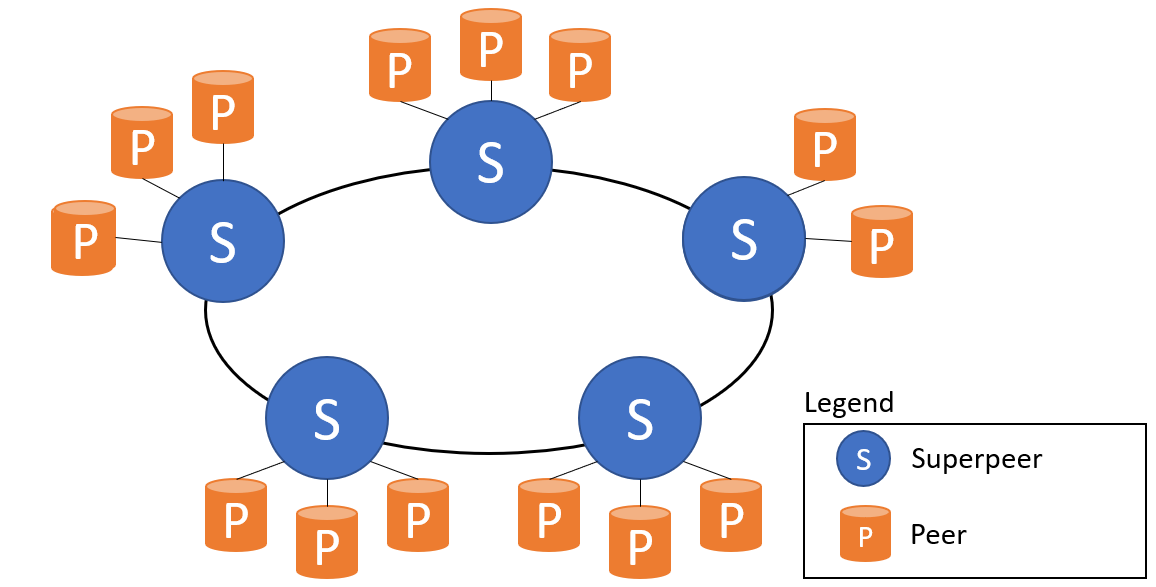
\includegraphics[width=1.0\linewidth]{img/topology.png}
	\caption{Topology of DXRAM}
	\label{topology}
\end{figure}
Peers are always assigned to one superpeer (Fig. ~\ref{topology}). Superpeer take over administrative tasks within the distributed system while peers serve the role of storage and/or backup nodes.
DXRAM provides its own application programming interface through the following services. DXRAM uses a distributed file system, so every node can access every file. To access or start an application within DXRAM, its Jar file must be located in the "plugin" folder. Then it needs to be  configured to autostart in the configurations of DXRAM or started via the terminal application.\\
Applications get access through services to various different feature of the system, like access on the distributed in-memory key/value store, the ability to run jobs and task on specified peers or to invoke other applications.\\

\noindent{\textit{BootService}}\\
The BootService provides access to all nodes inside the system. It can retrieve the specified roles of each node and its unique id.\\\\
\noindent{\textit{ChunkService}}\\
The ChunkService provides access to the in-memory key/value store of DXRAM. It allows to create, get, put and remove Chunks. Chunks are data structures, which extend the \textit{AbstractChunk} class. Each chunk must specify its size in bytes and how its data gets serialized and deserialized to binary. To identify chunks they get assigned an unique id, which links them to a location of their current size in the key/value store. If their size changes, their linked key/value store size must be changed as well, so their current size can fit into the storage. There are multiple implementations of ChunkServices. One of them is the regular ChunkServices, who allows storing chunks on every storage peer of the network, but there is also ChunkLocalService, who stores every chunk on the executing peer.\\\\
\noindent{\textit{NameserviceService}}\\
The NameserviceService allows to assign a unique \textit{short} String key to a chunk and register its key globally, so if other peers request a chunk id for this key they get the linked id. This is useful for getting chunks which do not change their content, if they are needed on multiple peers.\\\\
\noindent{\textit{SychronizationService}}\\
The SychronizationService allows to register barriers on peers. Barriers are used to control the flow of an application on multiple peers. They can also be used to share data structures between peers. A barrier gets created, stored and assigned an unique string key under which it gets registered at the NameserviceService. Then the barrier can be loaded on every needed peer and peers can sign on the barrier with the SychronizationService. If a peer signs on a barrier, it signals that it reached this point of the code and can optionally wait for the time critical tasks to end on all other peers. If all peers reached this point, they get notified and can continue.\\\\
\newpage
\subsection{Integration in DXRAM}
There are four main methods of integrating foreign code into DXRAM. There are application, jobs, task and functions. Applications are started through an autostart entry in the DXRAM configuration file or via the DXA-Terminal[?] application. There can only be a single instance of an application per peer. Applications are a good method of starting foreign code in DXRAM due to the lacking possibilities of starting jobs, task and functions, which is intended.\\
Jobs are a method to run foreign code on local and remote peers. Each peer got a local job queue and a pool of workers, who execute jobs of this queue based on a work stealing approach. Jobs do not offer a way of starting them without an application or an other method invoking them. For remote deployment, jobs must be able to be serialized.\\
The next approach are tasks. Task run on a computing group, which can be accessed through the \textit{MasterSlaveService}. It is lead by a peer, who is the master of this group. The master coordinates the whole computing group and takes over administrative tasks. Tasks can only be run on computing groups. This makes them more inflexible then jobs, which can be executed on any peer without setting up computing groups.\\
The last method is a distributed function, these functions get send to remote peers with their parameters and then their computation results gets returned to the invoking methods.
\begin{figure}[H]
	\centering
	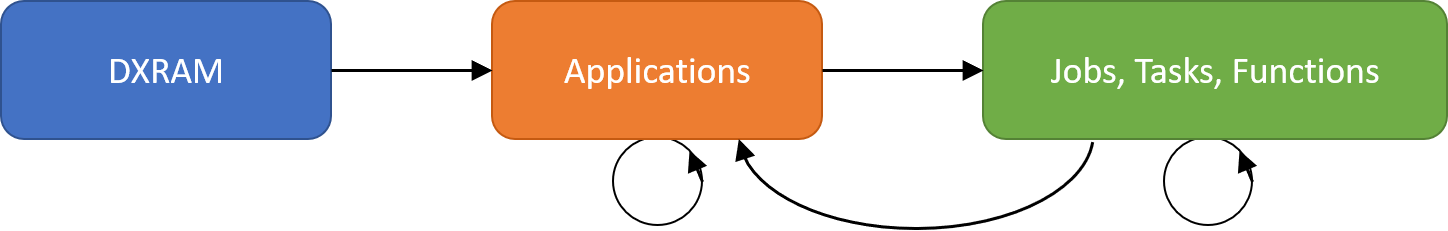
\includegraphics[width=1.0\linewidth]{img/codeintegration.png}
	\caption{Schema of Foreign Code Execution in DXRAM}
	\label{codeintegration}
\end{figure}

As shown in Fig.~\ref{codeintegration} applications are needed to execute jobs, tasks and functions. For the graph loader application jobs must be used to utilize multiple peers, as to the fact that it is too much effort to set up a computing group. Also graph loading is an operation, which is probably executed once. The graph loader must be a job to provide the possibility to integrate the graph loader into other projects. For direct access within DXRAM the graph loader job will be wrapped by an application. This can be seen in Fig.~\ref{integration}. This allows other projects to start the graph loader as job and avoiding application chaining. Due to the fact that jobs can invoke each other, exists the possibility to start multiple jobs on local and remote peers.

\begin{figure}[H]
	\centering
	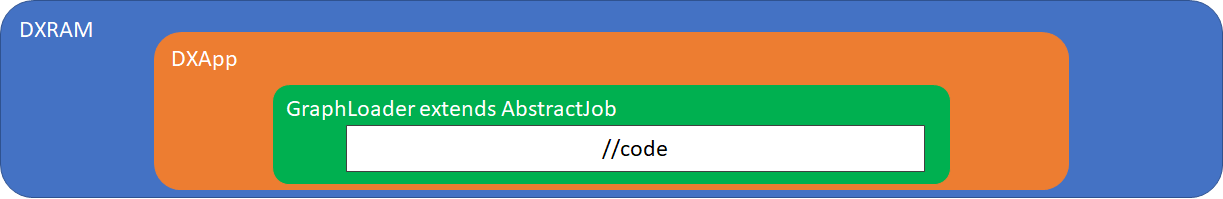
\includegraphics[width=1.0\linewidth]{img/schema.png}
	\caption{Schema of Integeration of the Graph Loader in DXRAM}
	\label{integration}
\end{figure}
\newpage
\section{Architecture of the Application}

There are two main task which could use speeding up. The first task is reading the ifle from disk and second is parsing the file and storing its data. A single machine will have much faster read speed from disk, due to fact that no data transmission between peers is needed. Therefore the loading into memory and distribution inside the distributed system, maybe slower then on a single machine. But this reading speed is depend on many factors, like the hardware and the implementation of the input methods. The main target is to speed up the performance of the parsing and storing of the graph, while equally distributing it into the in-memory system. As show in Fig.~\ref{loadingparsing} is the impact from parsing approximately 10 times higher then the impact from reading. Parsing the file is a computing intense task and suits the design of a distributed system.

\begin{figure}[H]
	\centering
	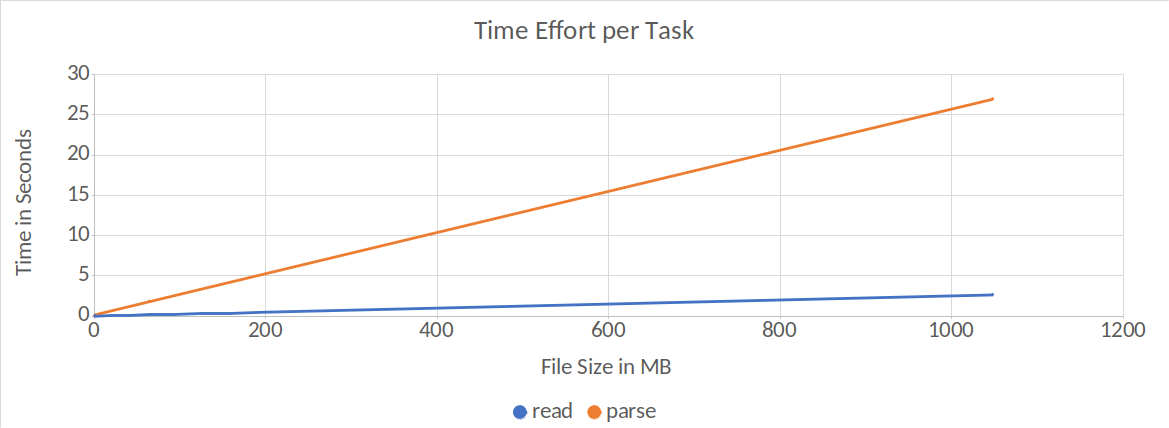
\includegraphics[width=1.0\linewidth]{img/tasktime.png}
	\caption{Local Single Threaded Benchmark of Loading and Parsing of different sized Graphs in Edge List Format for a Single-Pass Step}
	\label{loadingparsing}
\end{figure}

\subsection{Data Structures}
Sharing data structures between peers was not as straight forward as expected. Duo to the fact that the size of the graphs and their data structure grew at the same ratio. This lead to the problem of time outs of the networking component, when storing these structures in chunks on remote peers. To address this problem an layer of indirection was introduced, to divide the big chunks into smaller sections. Therefore, two dimensional arrays where needed. 
Also a wrapper class for the graph was need, it consist out of a set of vertex maps for each peer, which can also be stored in a chunk. The id of the graph object gets returned at the end of the graph loader, to provide access to following applications.\\
Apart from the chunk data structures, there were some important things to consider. Sections with data structures which get changed and accessed, should be thread safe for multiple job usage. There for \texttt{ConcurrentHashMaps} were used and \texttt{Lock}s to prevent jobs from interfering with each other. Also a queue was used for the chunks, which containing the file data, were removing elements also had to be thread safe.\\
For sending edges between peers, the wrapped maps could not be used, as maps are based on a unique key, which does not suit edges. Therefore, two arrays with linked entries were used to send edges between peers.\\
First linked lists were used for parallel reading chunks with file data were each chunk identified the next one. This approach was quite unstable, due to busy polling of the chunks on remote peers. The time gain of three seconds per gigabyte, did not make up the instabilities of busy polling on remote peers.\\

\subsection{Deployment of File data on nodes}
The distribution of the data inside the distributed system, will be done in three steps. The first step is to load the file into memory. DXRAM provides an network file system (NFS). So every peers could access and request files via network even if it is not physically on this peer. There are several methods of file interaction which could be used and need to be considered.

\subsubsection{Efficient Loading of File into Memory}
One key ability of the application is that the loading of the file system should be fast. Often the reading/writing from Storage Devices is a bottleneck. The first problem is that most Storage Devices are designed for sequential read and write operations and often support only one operation at a time. This leads to the problem that multiple threads reading the same storage device is a waste of performance and will not speed up the input rate of the file. Another problem is that accessing a storage device will cause a context switch. This results in the application stopping, while the kernel executes sensitive functions. This problem is often address with buffering the files and by requesting more data then needed in one step. Buffer sizes are one optimization problem to consider. [5]\\
The traditional way of accessing the data of a file is a common routine. First the file gets opened after that the data can be read, written in sequential or random order. This method causes many context switches, which force the application to stop, while the kernel executes sensitive functions. That is why in nearly every case IO gets buffered, so the context switches occur less often. [6]\\
This problem is addressed by memory mapping and suits large files where the context switches can be reduced drastically. A virtual memory mapping between the file system and the application address space is created. So expansive system calls can be avoided. The setup of this method is more expensive then the setup of a file reader. [5,6] But on the other hand mapped memory takes longer to setup and consumes more memory. Also Java does not offer the ability to free the mapped memory region which could lead into problems. For that reason traditional file concept will be used, so that the remaining memory map does not occupies storage space.

\subsubsection{Splitting and Distributing the File}
The deployment of the data can be done in multiple ways for this consideration network traffic gets ignored as it occurs in every implementation. Factors to consider are buffer sizes and other optimizations.\\

	\textit{Splitting into multiple smaller Files}\\
	One option would be to spit the huge into multiple files. This would result in maybe one file for each peer, which participates in our loading process, which can be access via the NFS and then be loaded. this approach simple to implement, but comes with some flaws. One down side is that the files gets read into memory then gets written in parts onto disk again, so it can be accessed on other peers. This would result in another reading/writing cycle and the NFS can not be controlled through the provided services API of DXRAM. Therefor, there could still be some problems with accessing a file located on the same storage device. Also the peers must read in the newly created small file again. This would result in $O(2n)$ for reading and writing and $O(\frac{n}{peers})$ on every peer for reading again.\\
	
	\textit{Splitting into small Chunks}\\
	This approach would generate memory chunks with our file data and distribute them via the \texttt{ChunkService}. There are two option chunks could be the size of $\frac{n}{peers}$ but this would result in the last peer waiting $O(n-\frac{n}{peers})$. This could be an big impact for many peers and very large files. To address that issue, a chunk size gets introduced  it can be small but variable to avoid splitting in contiguous regions. So the waiting gets reduced to $O(chunk \times peers)$ and they can start working as soon as possible. The total time taken to read the file is again $O(n)$ but writing to disk is not needed and the data is kept in memory, so reading it from disk is not needed either.
	While the chunks are created, the chunks could already be processed on the remote peers, so that the concurrency reduces the loading time.\\
	
	\textit{Reading via NFS}\\
	This approach would be slow and inefficient, due bottlenecks on the peer where the file is located and multiple peers causing random access patterns on the disk itself.\\

Splitting the file into chunks seems to be the best approach and will be featured in this work. This could also be optimized by starting to read vertices, while still distributing chunks onto other peers. Therefor the reading peer must approximate its own distribution, to process files.

\subsection{Processing/ Parsing of Data}
Each chunk will be reading separately and can not be depend on other chunks. This results in the fact that all data for interpreting this chunks must be provided by itself. Therefore, a parser must operate on each line of the format to interpret it and extract vertices or edges. Parser for other formats can be added easily by following the structure of the given ones.\\
Often a format is pretty similar to an other already implemented format, so the existing parser can be adjusted to suit a new format and be added to the loader application. Often parsers can be used to according ot other already implemented formats.
The processing/ parsing of the data is unique for each format. Some formats like the TGF need a a different parser in contrast to XML or JSON sytle formats. it can be assumed that the algorithm, which needs the data. Can not proceed without a complete dataset. Therefore most of the peers have no computing task, so that their computing power is available for loading the format. This results in the ability to create many heavy working threads to use all cores of the peers to their maximal capacity.

\subsection{Storing}
The extracted vertices, edges and optional metadata needs to be stored. For this task the \texttt{ChunkService} will be used to push the created structs into the key/value-store. ne problem of the distrubuted loading is that peers cannot wait on other peers to get information about vertices, because this would result in too much messages and network traffic for large datasets. This still leaves the problem of not synchronized vertex objects on different peers, which cant be written to the key/value-store because their information could be incomplete. 
\subsubsection{Duplicate node objects}
Some formats (especially in edge lists) nodes just get described by their edges. One problem is if two different peers create the same nodes by different edges, so they do not know if other peers already created a node object for specific nodes. As result they create a local node object with the information they got. In that case after reading the file in its entirety some merge of all hash maps and objects would need to be done. This would result in the problem that one assumption of this work is that one peer ca not keep all nodes and edges in memory, because there are too many objects.\\
Hash-Distribution of the Nodes while reading\\
As result of the fact of reorganizing the nodes after they have been loaded is very inefficient and does not suit our needs, the next approach would be to organize the nodes at loading/parsing-time.
One way could be to hash the labels/ids used in the graph. Note that the hashes created have no security constrains and do not need to be unique. This hash could be used to divide the nodes onto the peers. As result every peer would buffer all nodes, that do not belong to its range of hash values, and send the information he gathered to the according peers. This way we do not have to deal with duplicate nodes or merge. One problem of this approach is, that peers could end up with a chunk, that contains no nodes that hash to itself.\\
Hash-Distribution after reading\\
The peers could finish reading the nodes of its chunk and create their own versions in their key-value store. After reading and parsing is finished, they could like in first solution send the key-value-objects to the according nodes based on the hashes of their ids. The target peer then merges all versions of that node and stores the copy that has all information, the other duplicates get deleted. This could result in many objects for one node for each peer

\section{Issues}
A requirement is that the file is located inside one of our peers storage devices and is not part of our distributed system in any way. Loading files via an internet connection, will not be featured. Some start parameters are indispensable for this type of application, like the absolute file path, the format of the file or rather the parser that should be used and the number of peers to load the file.
Frist one peer should deal with the file, to distribute it to our others peers. The best thing would be, if the peer, who deals with file, would be the same peer where the file is located on. Otherwise the file transfer to the according peer would be a waste of time, especially for file sizes of several gigabytes. After the file chunks got deployed on the network, they could be parsed and loaded by the prior assigned peers into our DXRAM key-value store. [4]


First the file data gets loaded into small chunks which can be distrubted tFirst the file gets partially mapped into the memory, where it can be read by the master slave. The master slave first deals with the format specifications of the file, providing the division schema for splitting the file into chunks. chunks and will be dealing with the file format. Due to the fact that the data, is in memory, multiple thread can access the data parallel to accelerate processing. The processed data will be collected in chunks which will be deployed to the assigned slaves.
The support of infiniband would be increasing the performance drastically, due to spreading the data in the distributed system would be faster.
When the chunks arrive on the according slaves, they could immediately start processing their chunks.
 
Due to fact that some formats specify data of nodes in two or multiple places inside the file, it would be an interesting approach of using for example two memory maps of the same file in different sections. So, the chunk (buffer) can be filled with both information at the same time and the node information lie on all on one slave.

\newpage
The loading of graph formats consist out of a \textit{Two-Pass-Step} based approach for distributed systems. Therefor the application will be split up into mutiple loading stages, which will alternate between loading, creating and resolving cycles which can be seen in Fig. ~\ref{stages}.
\begin{figure}[H]
	\centering
	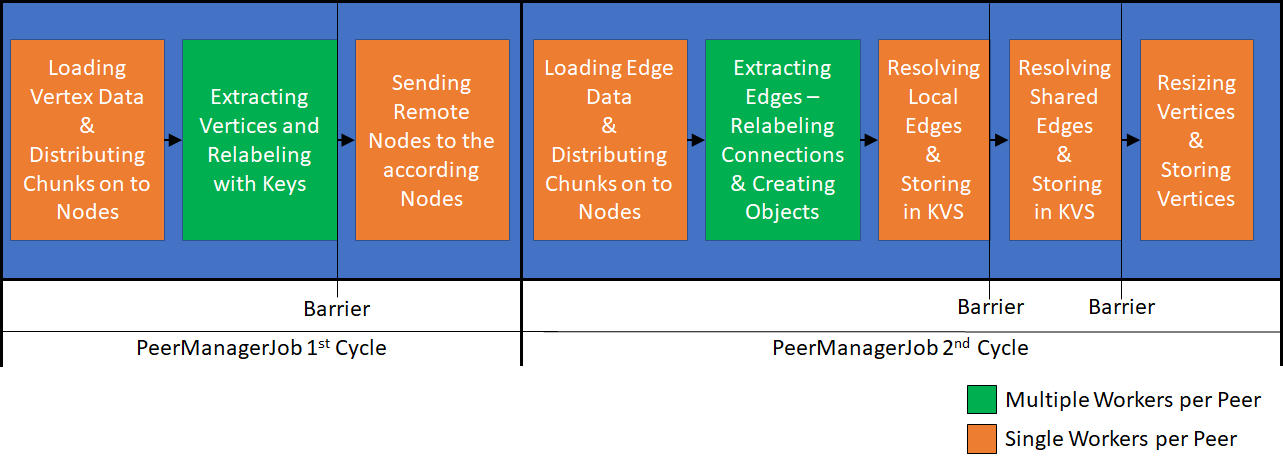
\includegraphics[width=1.0\linewidth]{img/schema_jobs.png}
	\caption{Stages of the GraphLoader Job}
	\label{stages}
\end{figure}

\section{Application Programming Interface}
The loader application provides an simple API. To add own formats, the class needs to be added to the \texttt{SupportedFormats} class and extend the \texttt{GraphFormat} class, which provides information of the required splitting type of the format and, how it should be read.
\subsection{SupportedFormats}
The \texttt{SupportedFormats} class, is the lookup table for all formats and which loader and splitter to use. It provides three simple functionalities.
\begin{itemize}
 \item[] \textit{addFormat(String key, Class$<$? extends GraphFormat$>$ format)}\\
 This function adds a format to the supported formats by assigning a key to a class type. For example ''{edgellist}'' is the key for the class \texttt{EdgeListFormat}.
 \item[] \textit{getFormat(final String key, final String[] files)}\\
 This function returns the class file for a given format key.
 \item[] \textit{isSupported(String key)}\\
This methods returns if a given key is supported.
\end{itemize}

\subsection{GraphFormat}
To add a custom format, the class needs to extend the \texttt{GraphFormat} class. A custom format specifies a Splitter and a Parser.
%First, a basic graph implementation with vertices and edges must be provided, those should be extendable due to different graphs, vertex and edge requirements of each format and application.
%Then the graph file will be split by lines for mostly likly simple graph file formats or interpreted for more complex ones. Out of those file splits - file chunks will be created which will be deployed to the corresponding peer. The peer will run the loading job with the loader provided for the format. The file format will be specified by the user as paramter.

%\begin{figure}[H]
%	\centering
%	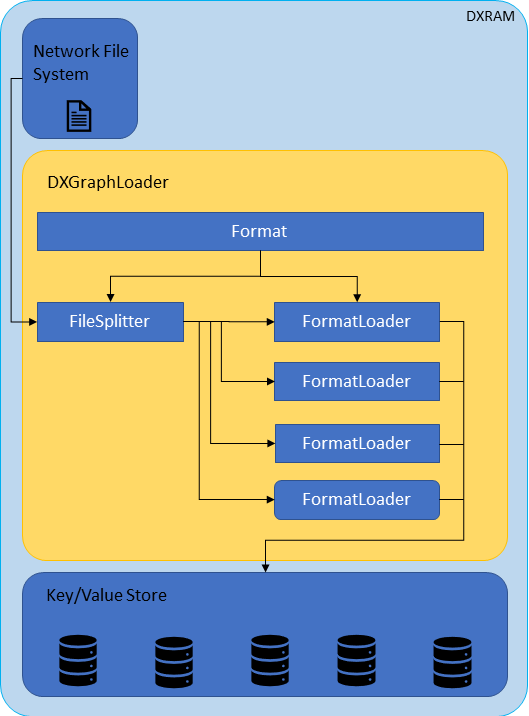
\includegraphics[width=1.0\linewidth]{img/layout.png}
%	\caption{Topology of DXRAM}
%	\label{topology}
%\end{figure}
\chapter{Evaluation}
\label{Evaluation}


%\section{Benchmark: File Reading Methods}
%\label{FileReading}
%Three diffrent methods where tested.  The first method utilizes the Java \texttt{Stream} api, to stream the lines of the file. This resulted in a short and intuitiv way of file handeling. The second method uses a \texttt{BufferedReader}, this method was also very easy to set up and reading files by line is a native function. RThe last method was java's implementation of mapped memory. At first the implementation this work would be based on wasn't faster then the other methods, duo to searching in Arrays and String for newline characters. The final implementation iterates over a char buffer provided by the \texttt{MappedByteBuffer} API and retuns a String.
%\begin{figure}[H]
%\centering
%  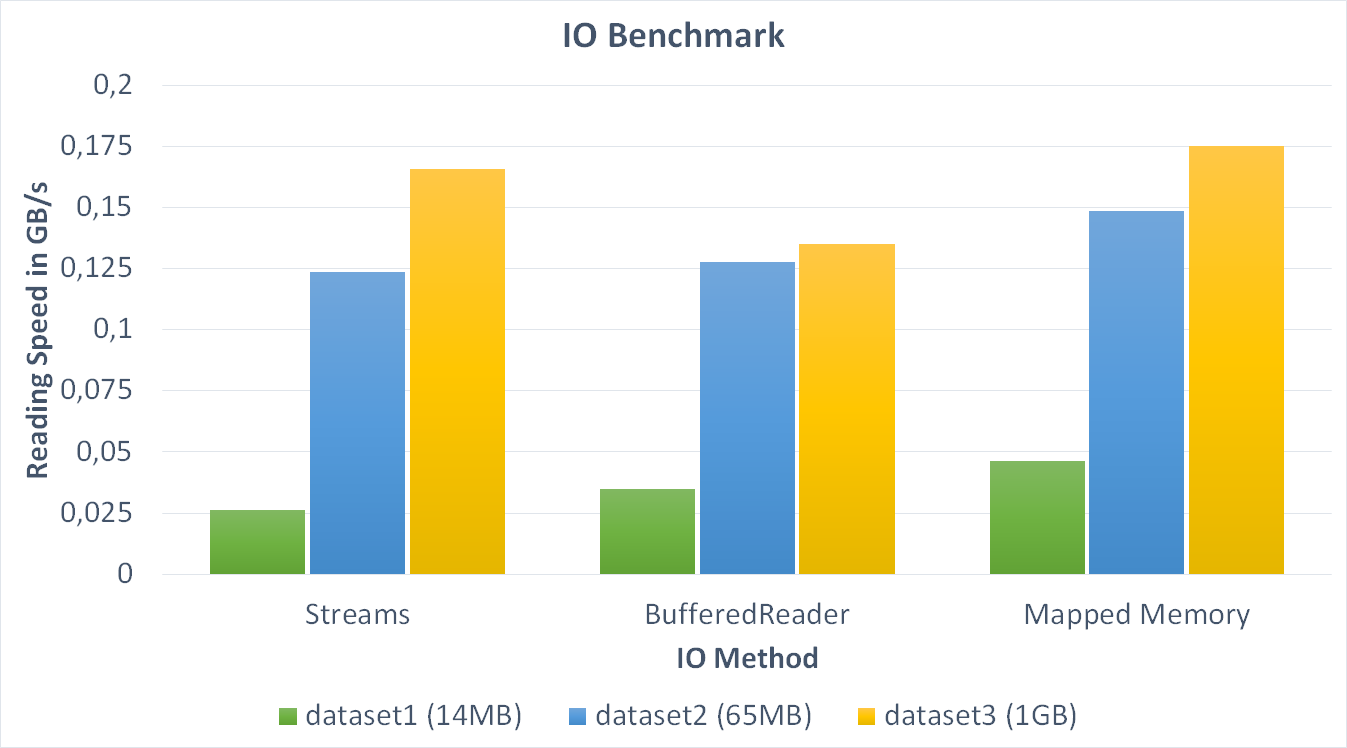
\includegraphics[width=1.0\linewidth]{img/iobench.png}
% \caption{IO Benchmark for File reading in Java}
%  \label{iobench}
%\end{figure}
%The resut of these optimizations can be seen, mapped memory is (not by far) the fastest method, for byte wise input mapped memory was by far the fastest. It can be seen that for the small files from dataset1 the initialization cost is very high compared to the total time taken, but when reading larger files, the initialization seems to be constant and it can be seen that the reading speed converges.
\chapter{Conclusion}

\end{abschlussarbeit}
\end{document}

